
\subsection{Answers}
\begin{table}[htb]%
\begin{center}%
\caption{Q29: In the tradeoff between code portability and performance, which is more or less important for you to write MPI programs? ["1" means portability is the most important and "3" means both are equally important.]}%
\label{tab:Q29-ans}%
\begin{tabular}{l|l|r}%
\hline%
Choice & Abbrv. & \# Answers \\%
\hline%
1 & Portability & 42 (5.1\%) \\%
2 & 2 & 93 (11.3\%) \\%
3 & 3 & 318 (38.7\%) \\%
4 & 4 & 252 (30.7\%) \\%
5 & Performance & 117 (14.2\%) \\%
\hline%
\multicolumn{2}{c}{total} & 822 \\%
\hline%
\end{tabular}%
\end{center}%
\end{table}%


In complement to the previous question, here, we look at the trade-off between
performance and portability. In this case, the outcome is clear. Even, if the
most given answer is somewhere in the middle-ground between maintaining
portability and providing better performance (3) with 38\%, the tendency is
highly towards improving performance (44\%) versus maintaining portability
(18\%). This may mean that the question of performance is more important because
applications are executed several times on a machine and that tuning it for
performance is more important than having users/developers spend some small
amount of efforts to update the application to a newer MPI API when moving from
one machine to a different one (as this occurs less often).  

\begin{figure}[htb]
\begin{center}
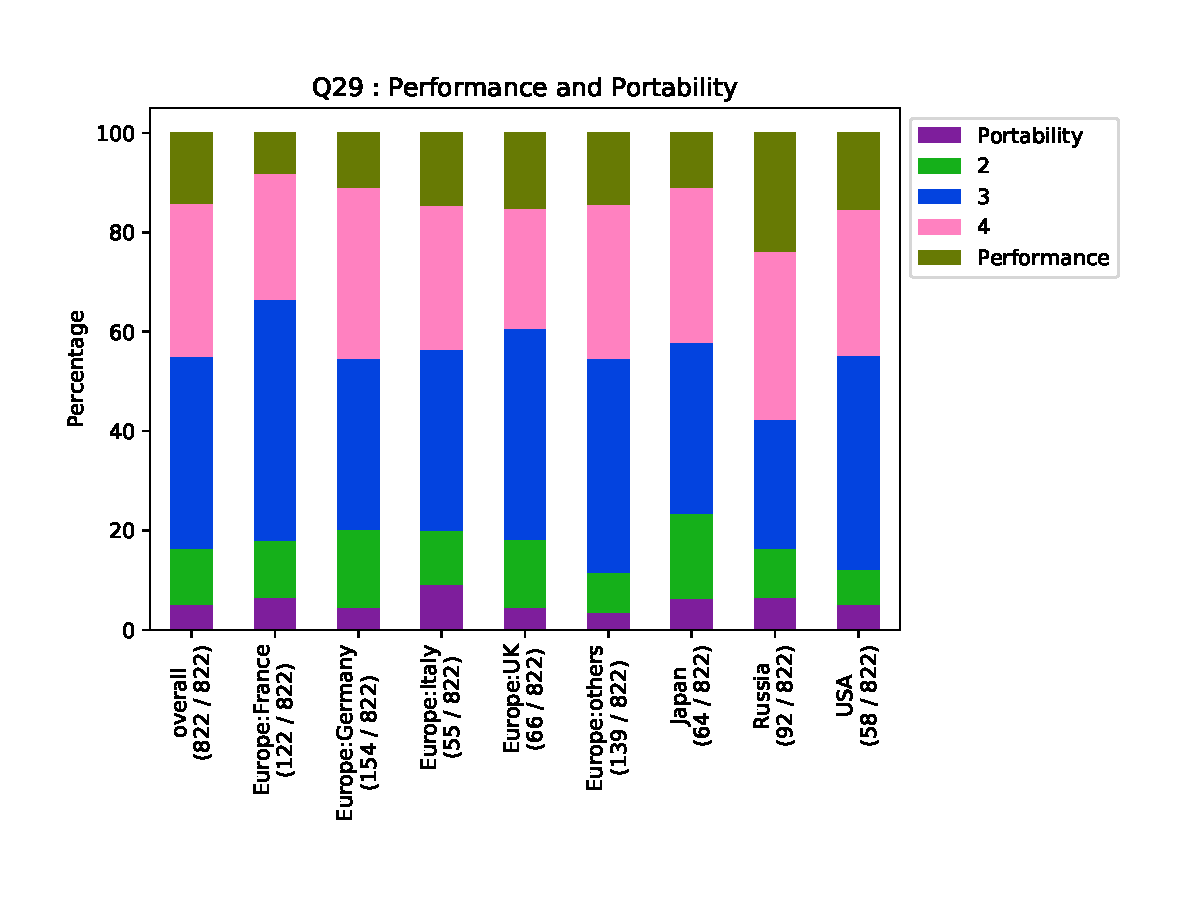
\includegraphics[width=10cm]{../pdfs/Q29.pdf}
\caption{Simple analysis: Q29}
\label{fig:Q29}
\end{center}
\end{figure}

Here, we should have the cross tab graph of Q28 and Q29. According to
the cross tab graph, many people said that MPI should maintain
backward compatibility in Q28, however, many of them also answered
that the compatibility and performance are equally important.
